We can now phrase the correctness properties in \autoref{sec:concepts} in terms
of the QAC language family:
\begin{enumerate}
  \item A rejection-sound ({\it i.e.} acceptance-complete) validator consumes
    all traces that are producible by the protocol specification:
    \[\begin{array}{lrl}
      \rejSound v s&\triangleq&\forall t,\rejects v t\implies\invalid s t\\
      &\triangleq&\forall t,(\exists s',\behaves s t s')\implies\exists v',\behaves v t v'
    \end{array}\]
  \item A rejection-complete ({\it i.e.} acceptance-sound) validator only
    consumes traces that are producible by the protocol specification:
    \[\begin{array}{lrl}
      \rejComplete v s&\triangleq&\forall t,\invalid s t\implies\rejects v t\\
      &\triangleq&\forall t,(\exists v',\behaves v t v')\implies\exists s',\behaves s t s'
    \end{array}\]
\end{enumerate}

Both the specification and the validator are infinite loops.  To show that the
validator consumes the same space of traces as the specification produces, we
need to show the correspondence between each server and validator step.  This is
done by introducing some loop invariant between the server and validator states,
and show that it is preserved by the server's and the validator's loop body.

\subsection{Proving rejection soundness}
To prove that any trace producible by server $\existT{S}{\sigma}{(\sstep,s_0)}$
is consumable by validator $\existT{V}{\beta}{(\vstep,v_0)}$, I perform forward
induction on the server's execution path, and show that every step has a
corresponding validator step:
\begin{itemize}
\item The initial server state $s_0$ simulates the initial validator state $v_0$:
  \begin{equation}
    \tag{RejSound-Init}
    \label{eq:rs1}
    \Reflects{(v_0:\beta)}{(s_0:\sigma)}
  \end{equation}
\item Any server step $\sstep(q,c,s)=(a,s')$ whose pre-execution state $s$
  reflects some pre-validation state $v$ can be consumed by the validator
  yielding a post-validation state $v'$ that reflects the post-execution state $s'$:
  \begin{align*}
    \tag{RejSound-Step}
    \label{eq:rs2}
    &\forall(q:Q)(c:C)(a:A)(s,s':\sigma)(v:\beta),\\
    &\sstep(q,c,s)=(a,s')\wedge\Reflects{v}{s}\\
    &\implies\exists v':\beta,\vstep(q,a,v)=\Some{v'}\wedge\Reflects{v'}{s'}
  \end{align*}
  \begin{center}
    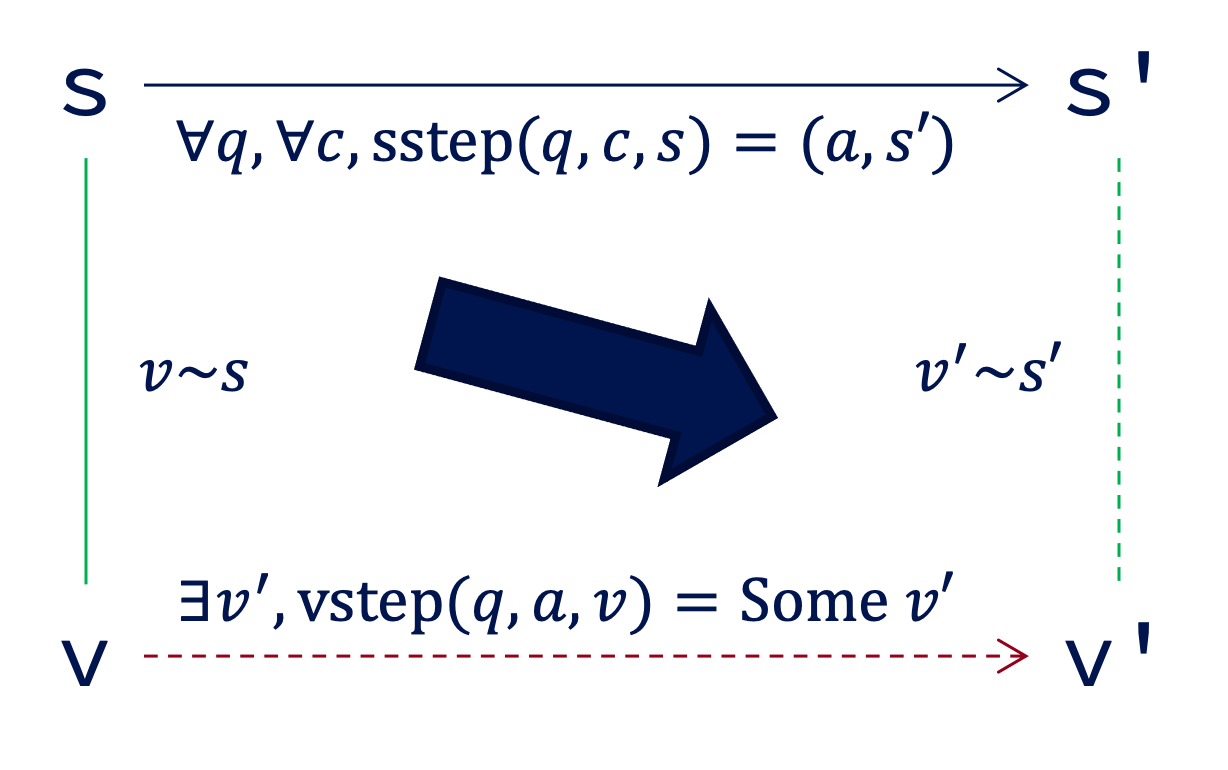
\includegraphics[width=.5\textwidth]{figures/sound}
  \end{center}
\end{itemize}

\subsection{Proving rejection completeness}
To prove that any trace consumable by validator
$\existT{V}{\beta}{(\vstep,v_0)}$ is producible by server
$\existT{S}{\sigma}{(\sstep,s_0)}$, we need backward induction on the
validator's execution path and show that every step has a corresponding server
step:
\begin{itemize}
\item Any accepting validator step $\vstep(q,a,v)=\Some v'$ has some server
  state $s'$ that reflects the post-validation state $v'$:
  \begin{align*}
    \tag{RejComplete-End}
    \label{eq:rc1}
    \forall(q:Q)(a:A)(v, v':\beta),\;&\vstep(q,a,v)=\Some{v'}\\
    &\implies\exists s':\sigma,\Reflects{v'}{s'} 
  \end{align*}
\item Any accepting validator step $\vstep(q,a,v)=\Some v'$ whose
  post-validation state $v'$ reflects some post-execution server state $s'$
  has a corresponding server step from a pre-execution state $s$
  that reflects the pre-validation state $v$:
  \begin{align*}
    \tag{RejComplete-Step}
    \label{eq:rc2}
    &\forall(q:Q)(a:A)(v,v':\beta)(s':\sigma),\\
    &\vstep(q,a,v)=\Some{v'}\wedge\Reflects{v'}{s'}\\
    &\implies\exists(s:\sigma)(c:C),\sstep(q,c,s)=(a,s')\wedge\Reflects{v}{s}
  \end{align*}
  \begin{center}
    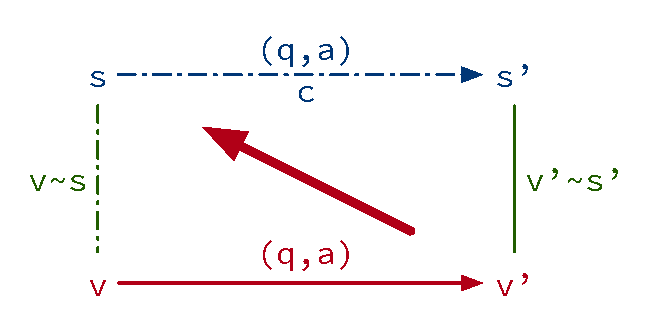
\includegraphics[width=.5\textwidth]{figures/complete}
  \end{center}

\item The initial validator state $v_0$ only reflects the initial server state $s_0$:
  \begin{equation}
    \tag{RejComplete-Init}
    \label{eq:rc3}
    \{s\mid\Reflects{v_0}{s}\}=\{s_0\}
  \end{equation}
\end{itemize}

Rejection soundness is proven by forward induction, while rejection completeness
is proven by backward induction.  This is because the choice $C$ is known from
the server step, but unknown from the validator step: Given a validator step, we
cannot predict ``what choices the server will make in the future'', but can
analyze ``what choices the server might have made in the past''.  This proof
strategy is further explained with the $\Prog$ example.
